%!TEX root = usersmanual.tex
\chapter{\textsc{Examples}}
	\section{Gene Expression with Fluorescent Reporter (\texttt{geneexpr})}
		\subsection{Overview}
		This example shows constitutive expression of the destabilized enhanced Green Fluorescent Protein (deGFP) from a gene on a plasmid. It shows one of the simplest circuits that can be modelled with the modelling toolbox, and in doing so, illustrates its basic features. These include displaying the evolution of the expressed protein (deGFP) levels, resource usage (Amino Acids (AA) and Nucleotide Pairs (NTPs)), the evolution of the DNA and mRNA concentrations. Figure \ref{fig:geneexpr schematic} shows a schematic of this circuit. \\
		
		\begin{figure}
		\begin{center}
		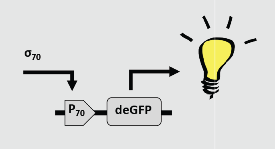
\includegraphics{geneExpr schematic.png} 
		\caption{Schematic of the gene expression circuit'}
		\label{fig:geneexpr schematic}
		\end{center}
		\end{figure}		
		 
		% show a figure with p70 promoter, rbs, DNA, leading to protein. 
		The diagram shows the DNA made of the p70 promoter, the most common constitutive promoter in the toolbox, followed by the deGFP gene. The gene is then transcribed into mRNA which is translated into DNA. 
		\ref{fig:geneexpr} shows the output plot for this example. 
		
		
		
		\subsection{Walk-through}
		If you have not already done so, ensure that you are in the \textsf{\textbackslash trunk} directory, and run \texttt{txtl\_init} to add the necessary directories to the MATLAB search path. 
			
		The first step is to decide on a extract to use. The extract contains RNAP, Ribo, $\sigma 28$ and $\sigma 70$, RecBCD, RNA-ase, and sets up the reactions for the formation of RNAP70 and sequestration of RecBCD. The extract we will be using will be created using parameters defined in the external configuration file \textsf{'E15\_config.csv'}, and is implemented as: 
		
				\begin{flushleft}
						\texttt{tube1 = txtl\_extract('E15');} 
				\end{flushleft}	
				
				Note that this command returns a handle to a Simbiology model object. This is stored in the aptly named variable \texttt{tube1}. We will later combine the 'contents' of this tube with those of other tubes, just like we do in the experimental protocol. One may read about Simbiology model objects at \url{http://www.mathworks.com/help/simbio/ug/what-is-a-model.html#bsrhh1k} and \url{http://www.mathworks.com/help/simbio/ref/modelobject.html}.
				
Next, we define the buffer (containing AA and NTP) to use, and store it in \texttt{tube2}. Once again, the buffer contents are drawn from the configuration file \textsf{'E15\_config.csv'}:

				\begin{flushleft}
						\texttt{tube2 = txtl\_buffer('E15');} \\	
				\end{flushleft}	 
		
We then use the \texttt{txtl\_newtube} command to create a new model object which will contain the DNA we wish to use. This is done as follows:
		
				\begin{flushleft}
						\texttt{tube3 = txtl\_newtube('gene\_expression');} \\	
				\end{flushleft}	 
				
The next step is to define the DNA sequences to be added to \texttt{tube3}. This is done using the \texttt{txtl\_add\_dna} command:

				\begin{flushleft}
						\texttt{dna\_deGFP = txtl\_add\_dna(tube3, 'p70(50)', 'rbs(20)', 'deGFP(1000)', 1, 'plasmid');} \\	
				\end{flushleft}
Refer to the description of the \texttt{txtl\_add\_dna} command in \S 3.2 for full details of its usage. For our purposes, it suffices to know that this DNA is loaded onto a plasmid, and contains a p70 promoter (constitutive, 50 base pairs (BP) in length), a 20BP RBS domain, and a 1000BP deGFP gene. Furthermore, the DNA is such that the \textbf{final} concentration of this DNA in the \textbf{combined} tube will be 4nM. 

We then simply combine the extract, buffer, and DNA:

				\begin{flushleft}
						\texttt{Mobj = txtl\_combine([tube1, tube2, tube3]);} \\	
				\end{flushleft}
							
We now have to set the amount of time we want our simulation to run for and calling the \texttt{txtl\_runsim} command as follows:	

				\begin{flushleft}
						\texttt{[simData] = txtl\_runsim(Mobj,14*60*60);} \\
						\texttt{t\_ode = simData.Time;}
						\texttt{x\_ode = simData.Data;}
				\end{flushleft}	
This call to \texttt{txtl\_runsim} takes the Simbiology model object and the experiment duration to be simulated, and runs the simulation from time zero to time 14 hours. It returns a \texttt{simData} object, from which we can extract a vector of time points in that range (\texttt{t\_ode}) and a matrix \texttt{x\_ode}, where each column is the concentrations of a species in the model at time points corresponding to \texttt{t\_ode}. For more information, please refer to \textsc{Chapter 3: Overview of the Core Processes}. 

Finally, the modelling toolbox contains a set of plotting tools that simplify the plotting of standard species, like Proteins, DNA, RNA and resources. We use \texttt{txtl\_plot} to accomplish this. One may simply call \texttt{txtl\_plot} with the data and model object as follows: \\

\noindent \texttt{txtl\_plot(t\_ode,x\_ode,Mobj); \\}

\noindent leading to a default set of species to be plotted. 
						
		\subsection{Results}
		
		Figure \ref{fig:geneexpr} shows the output of the plotting command for this example. The top plot shows the protein species present in the model, the bottom left plot shows the DNA and mRNAs in the system, and the bottom right plot displays the resource usage. We observe that deGFP almost entirely exists in the mature state, and rises constantly for the first 200 minutes, before reaching a steady state of about 2uM.\\
		
		
		\begin{figure}
		\begin{center}
		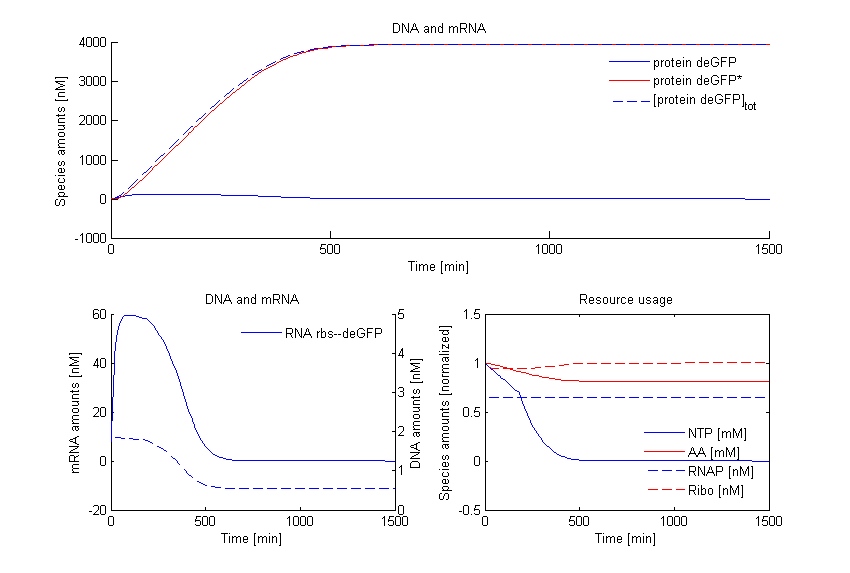
\includegraphics[width=\textwidth]{GeneExpressionPlotActuallyProducedByCode.png} 
		\caption{Gene Expression Output}
		\label{fig:geneexpr}
		\end{center}
		
		\end{figure}
		
%% NEGATIVE AUTOREG
	\section{Negative Autoregulation (\texttt{negautoreg})}
%%%% OVERVIEW	
		\subsection{Overview}
		Negative autoregulation refers to the repression of gene expression by a protein encoded by that very gene. In this code, we will show that dimerized tetR protein represses its own production, and thus leads to a relatively low steady state concentration. 
		\subsection{Code}
		Please work through the Gene Expression example above to get basic familiarity with the commands and their usage. This example is slightly more complex than \texttt{geneexpr}. We provide the entire code for this example below: \\
		
		\noindent \texttt{tube1 = txtl\_extract('E9');} \\
								\texttt{tube2 = txtl\_buffer('E9');} \\
								\texttt{tube3 = txtl\_newtube('negautoreg');} 
								\vspace*{1\baselineskip}
								
								\noindent \texttt{dna\_tetR = txtl\_add\_dna(tube3, 'thio-junk(500)-ptet(50)', 'rbs(20)', 'tetR(647)-lva(40)', 16, 'linear'); }\\
								\texttt{dna\_deGFP = txtl\_add\_dna(tube3, 'p70(50)', 'rbs(20)', 'deGFP(1000)', 16, 'linear');}\\
								\texttt{dna\_gamS = txtl\_add\_dna(tube3, 'p70(50)', 'rbs(20)', 'gamS(1000)', 1, 'plasmid');}
								\vspace*{1\baselineskip}
								
								\noindent \texttt{Mobj = txtl\_combine([tube1, tube2, tube3]);} 
								\vspace*{1\baselineskip}	
								
								\texttt{simulationTime =  8*60*60;}\\
								\texttt{[t\_ode, x\_ode, mObj, simData] = txtl\_runsim(Mobj, simulationTime);}
								\vspace*{1\baselineskip}
								
									 \begin{flushleft}
						 \texttt{\noindent txtl\_plot(t\_ode,x\_ode,Mobj); \\} 
						 \end{flushleft}
		
		The important differences from the gene expression examples are that here we add 3 pieces of DNA into tube 3, two of which are linear. \\
		The tetR DNA uses a ptet promoter, which is repressed by the tetR protein dimer. Attached to the ptet promoter, there are two domains (thiosulfate 'thio' and junk DNA 'junk) which lower the rate of DNA degradation by the exonuclease RecBCD. The tetR DNA also shows an 'lva' tag, which attaches a amino acid sequence to the tetR protein and marks it for degradation by the protease ClpXP. In a futire version, all the 'lva' tags will be replaced by the 'ssrA' tags, although for the functioning of this toolbox, this name change is inconsequential. The reaction rate parameters for ClpXP's action are currently in the process of being determined. \\
		The second DNA, deGFP, is just like in the gene expression exampe, except that in this case it is mounted on a 'linear' DNA, and therefore can be degraded. \\ 
		The third DNA, gamS, is mounted onto a plasmid, and is thus safe from degradation. GamS helps to sequester the RecBCD exonuclease, providing protection tot the DNA. \\
		%Note that as opposed to the plotting function in the gene expression example, here we call txtl\_plot without the data groups input, and so the plotting function uses the defaults. 
		
		
		\subsection{Results}	
		
		\begin{figure}
		\begin{center}
		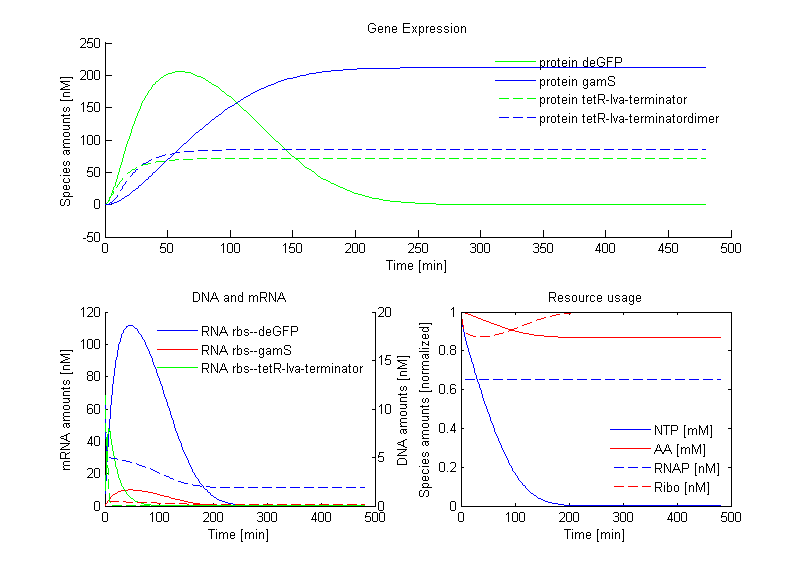
\includegraphics[width=\textwidth]{NegativeAutoregulationPlotActuallyProducedByCode.png} 
		\caption{Negative Autoregulation Output}
		\label{fig:negautoreg}
		\end{center}
		
		\end{figure}
		Figure \ref{fig:negautoreg} illustrates a number of features: expression of gamS, tetR and the tetR dimer, the respective mRNAs, and resources. The first thing to note is that expression levels in this example are an order of magnitude lower than in gene expression. There are two reasons for this: The use of 'linear' DNA, which means that RecBCD mediated DNA degradation is active, and the quick depletion of the RNA, due to the greater amount of RNA produced.  
		
	\section{Induction of Gene Expression using aTc (\texttt{induction})}
		\subsection{Overview}
		In this circuit, we explore the effect of varying levels of the inducer 'aTc' on the expression of a gene under the control of the tetR repressed ptet promoter. The expressed gene is precisely the tetR protein, leading to a negative autoregulation circuit as in the previous example. This DNA is loaded onto a plasmid DNA, and so no DNA degradation occurs. Figure \ref{fig:inductionSchematic} shows the circuit diagram for this example. Note that in the diagram, the deGFP and tetR are fused, while in the simulation, we only use the tetR gene, but we set its length to be 1200, comparable to the length of the tetR-deGFP fusion DNA. \\ 

		\begin{figure}
		\begin{center}
		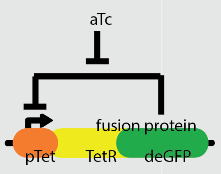
\includegraphics{negautoreg_induction schematic.png} 
		\caption{Schematic of the induction circuit'}
		\label{fig:inductionSchematic}
		\end{center}
		\end{figure}		
		
		 
		\subsection{Code}
		This code uses the \texttt{txtl\_addspecies} command to add increasing amounts of \texttt{'aTc'} to the model object, and executes the simulation. The Figure \ref{fig:induction} below plots the levels of tetR protein at different \texttt{'aTc'} concentrations. \\
		
		Set up tubes: \\
\noindent \texttt{tube1 = txtl\_extract('E6');} \\
\texttt{tube2 = txtl\_buffer('E6');} \\
\texttt{tube3 = txtl\_newtube('circuit');} 
\vspace*{1\baselineskip}
		
		Construct DNA and add to \texttt{tube3}: \\						
\noindent \texttt{dna\_tetR = txtl\_add\_dna(tube3, 'thio-junk(500)-ptet(50)', 'rbs(20)', 'tetR(1200)-lva(40)', 16, 'plasmid'); } \\
\texttt{dna\_gamS = txtl\_add\_dna(tube3, 'p70(50)', 'rbs(20)', 'gamS(1000)', 0, 'plasmid');}
\vspace*{1\baselineskip}
			
		Add protein gamS to the model. We used \texttt{txtl\_add\_dna} to set up its reactions. \\
		
		\noindent \texttt{gamS = txtl\_addspecies(tube3, 'protein gamS', 100);}
\vspace*{1\baselineskip}
				
		Define levels of \texttt{aTc} to use. \\						
\noindent \texttt{count = 1;}\\
% Do runs at different inducer levels
\texttt{levels = [0 2 5 10 20 40 100 300 1000];}\\
\texttt{colors = \{'r', 'b', 'g', 'c', 'm', 'y', 'k', 'r--', 'b--'\};}
\vspace*{1\baselineskip}
								
		Combine tubes: \\						
\noindent \texttt{Mobj = txtl\_combine([tube1, tube2, tube3]);}
\vspace*{1\baselineskip}
								
		Iteratively Simulate the model with different levels of aTc. \\						
\noindent \texttt{for atc = levels }\\
 \texttt{configsetObj = getconfigset(Mobj, 'active');}\\
  \texttt{set(configsetObj, 'StopTime', 6*60*60);  }\\
  \texttt{[t\_ode, x\_ode, Mobj, simData] = txtl\_runsim(Mobj, configsetObj); }
\vspace*{1\baselineskip}
								
\noindent \texttt{figure(2); hold on;}\\
  \texttt{itetR = findspecies(Mobj, 'protein tetR');}\\
  \texttt{plot(t\_ode, x\_ode(:, itetR), colors\{count\});}\\
  \texttt{labels{count} = [int2str(atc) ' nM aTc'];}
								\vspace*{1\baselineskip}
								
  % Add additional inducer for the next run
  \noindent \texttt{if count < size(levels,2)}\\
  \texttt{inducer = txtl\_addspecies(Mobj, 'aTc', levels(count+1)-levels(count));}\\
  \texttt{count = count + 1;}\\
  \texttt{end}\\
\texttt{end}
	\vspace*{1\baselineskip}
								
\noindent \texttt{title('Time Responses');}\\
\texttt{lgh = legend(labels, 'Location', 'Northwest');}\\
\texttt{legend(lgh, 'boxoff');}\\
\texttt{ylabel('Species amounts [nM]');}\\
\texttt{xlabel('Time [min]');}

		
		
		\subsection{Results}	
		\begin{figure}
		\begin{center}
		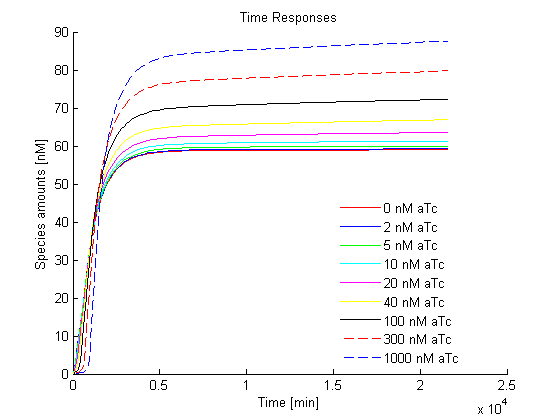
\includegraphics[width=\textwidth]{induction.png} 
		\caption{Induction of tetR expression due to aTc}
		\label{fig:induction}
		\end{center}
		
		\end{figure}
		Figure \ref{fig:induction} shows the concentrations of tetR. Note that this is not the standard plot generated in the previous two examples. We used the \texttt{findspecies} function to obtain the index of the species to plot (\texttt{[protein tetR]}) by using that index to access the relevant column of the data vector \texttt{x\_ode}. \\
		
		We note that as the \texttt{aTc} concentration is increased, the level of \texttt{tetR} in the system increases due to reduced repression of \texttt{ptet} by \texttt{protein tetRdimer}. 
		
%	\section{Incoherent Feedforward Loop (incoherent\_ff\_loop)}
%		\subsection{Overview}
%		\subsection{Code}
%		\subsection{Results}	